\chapter{L’exemple des myopathies congénitales et la difficulté du diagnostic}
Dans cette thèse, nous avons cherché à développer des méthodes \gls{ia} pour exploiter les données biomédicales. Nous nous sommes concentrés sur les données de patients atteints de myopathies congénitales: une famille de maladies des muscles rares et génétiques, dont le diagnostic est complexe. Dans ce chapitre, nous allons présenter le contexte biologique de ces maladies avec une présentation de la structure du muscle, de la classification des myopathies congénitales et de leur diagnostic.

\section{Le muscle, un organe particulier assurant des fonctions diverses}
Le muscle est un organe particulier tant par sa structure que par son abondance dans le corps humain. Pour un adulte, les muscles représentent près de 40\% de la masse corporelle totale (\cite{janssen_skeletal_2000}). Les muscles assurent une variété de fonctions, dont le mouvement et la posture, mais aussi la thermogénèse et l'équilibre métabolique.

Dans le muscle, divers processus sont nécessaires pour permettre d'assurer ses fonctions. Le muscle intègre des processus neurologiques pour le transfert de signaux induisant la contraction. Cette contraction est possible grâce à une structure particulière du muscle en fibres que nous présenterons en détail dans la section \ref{muscle_struc}. De plus, cette contraction requiert de l'énergie qui est fournie par des processus métaboliques. Enfin, le muscle, en raison des contraintes mécaniques subies lors des mouvements, est un organe dynamique dans lequel des processus de régénération musculaire sont à l'œuvre pour assurer sa plasticité.

\subsection{Types de muscles}
Il existe dans le corps humain trois types de muscles avec des structures différentes selon la fonction qu'ils doivent assurer (figure \ref{fig:muscle-type}, \cite{gomez_oca_physiological_2021}): le muscle lisse, le muscle cardiaque et le muscle strié squelettique.
\begin{figure}[!ht]
 \centering
 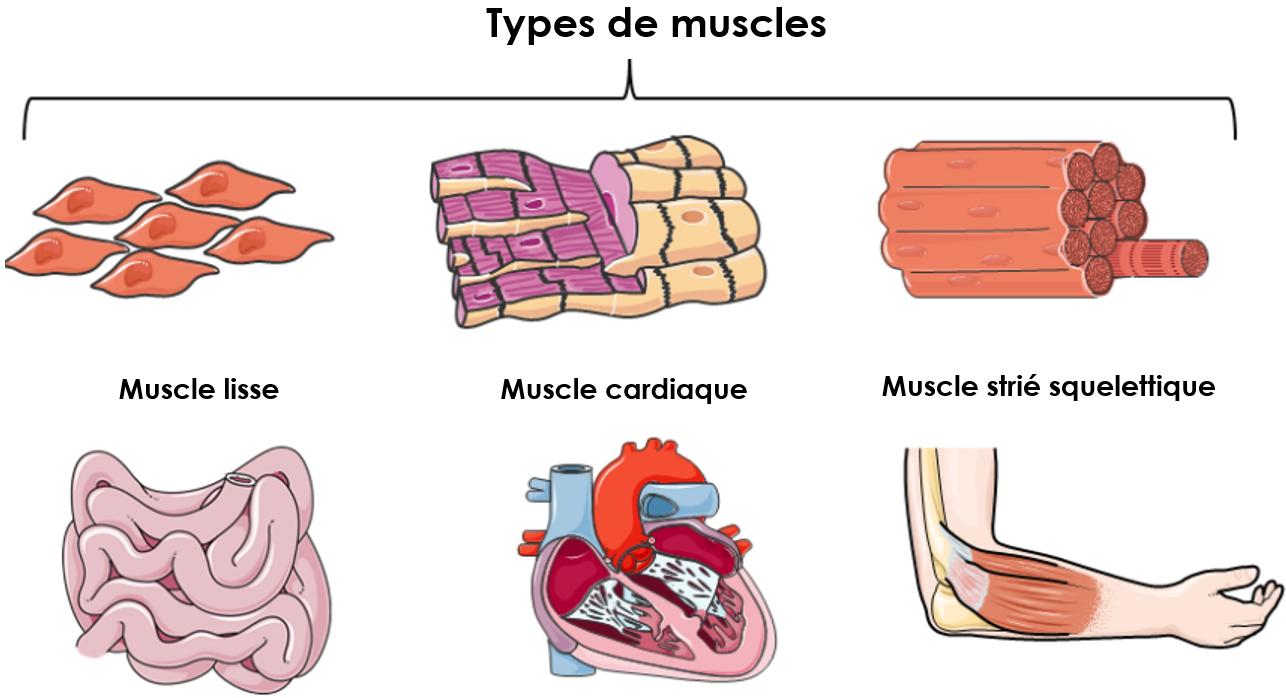
\includegraphics[width=0.8\textwidth]{figures/muscle_type.png}
 \caption[Schéma des trois types de muscles]{\textbf{Schéma des trois types de muscles}. Les muscles lisses se contractent de manière involontaire (vaisseaux sanguins, appareil digestif). Les muscles striés squelettiques se contractent de manière volontaire (mouvement du corps). Les muscles cardiaques sont aussi striés, mais se retrouvent uniquement dans le cœur et se contractent de manière involontaire et en rythme. (traduit de \cite{gomez_oca_physiological_2021})}
 \label{fig:muscle-type}
\end{figure}
\subsubsection{Muscle lisse}
Le muscle lisse, aussi nommé non strié tire son nom de l'absence de striations lors de l'observation au microscope. Les fibres ne possèdent qu'un seul noyau central. Ce type de muscles est présent dans la paroi de nombreux organes, tels que les vaisseaux sanguins, l'appareil digestif, l'appareil respiratoire, l'appareil urinaire et la paroi des viscères. La particularité des muscles lisses est qu'ils se contractent de manière involontaire, sans contrôle conscient. La contraction de ces muscles est régie par le système nerveux neurovégétatif (système autonome).

\subsubsection{Muscle strié cardiaque}
Le muscle strié cardiaque est un muscle qui se retrouve exclusivement dans le cœur. Il partage des caractéristiques communes à la foi au muscle lisse et au muscle strié squelettique. Ce muscle se contracte de manière involontaire, et les fibres ne possèdent qu'un seul noyau central à l'instar des muscles lisses. Cependant, le muscle cardiaque présente des striations similaires au muscle strié squelettique. La caractéristique unique du muscle strié cardiaque est qu'il fonctionne en continu et se contracte en rythme de façon coordonnée. Ainsi ce muscle est très dépendant du métabolisme oxydatif.

\subsubsection{Muscle strié squelettique}
Enfin, les muscles striés squelettiques, aussi nommés muscles volontaires, sont les muscles mobilisés lors des mouvements conscients et volontaires, lorsque l'on porte un objet ou que l'on fait du sport par exemple. Au microscope, ces muscles se démarquent par la présence de stries transversales et longitudinales. Les cellules composant les fibres musculaires du muscle strié squelettique ont la particularité d'avoir fusionné, formant ainsi un "syncitium vrai". Cette fusion donne donc aux fibres musculaires les caractéristiques des cellules géantes (entre 1 et 5 cm de long et 10 à 100µm de diamètre). Ainsi, ces cellules sont multinucléées avec des noyaux périphériques.

Comme leur nom l'indique, ces muscles sont reliés aux os par l'intermédiaire du tendon, leur contraction permet donc le mouvement des os et donc du corps. Cette contraction est engagée sous le contrôle du système nerveux somatique. En fonction de l'intensité et de la durée de la contraction, les muscles striés squelettiques peuvent fonctionner de manière aérobie grâce à leur vascularisation importante ou de façon anaérobie.

Dans le cadre des myopathies congénitales, les muscles striés squelettiques sont affectés et ne sont plus capables d'assurer leur fonction normale en raison d'altérations structurelles, entrainant un déficit de tonus musculaire et de force.

\subsection{Structure du muscle strié squelettique}\label{muscle_struc}
Pour comprendre comment les altérations de la structure du muscle observées dans les myopathies congénitales peuvent mener à son dysfonctionnement, il est important de comprendre comment le muscle est structuré et comment il peut se contracter.

L'organisation du muscle peut être décrite comme celle d'une corde d'escalade. Une corde d'escalade semble être composée d'un seul élément fort et résistant. Mais si l'on y regarde de plus près, une corde d'escalade est constituée d'une gaine qui entoure l'âme de la corde. Cette âme est composée de plusieurs gros filaments, eux-mêmes composés de plusieurs filaments de plus en plus fins, torsadés ensemble. 

Ainsi par analogie, le muscle entier est comme la corde d'escalade, sa structure est décrite dans la figure \ref{fig:muscle_struct} (\cite{burr_basic_2019}). Le muscle entier, entouré par sa gaine nommée \textit{epimysium} et \textit{perimysium}, est constitué de plusieurs faisceaux musculaires qui le composent. Chacun de ces faisceaux ou fascicules est composé de filaments encore plus fins nommés fibre musculaire. Ces fascicules et fibres musculaires sont encore observables au microscope optique. Enfin, chacune de ces fibres musculaires est en fait un regroupement de plus petits filaments nommés myofibrilles qui sont des filaments composés d'une multitude de myofilaments capables de se contracter. Les myofibrilles et myofilaments ne sont observables qu'en microscopie électronique.

\begin{figure}[!ht]
 \centering
 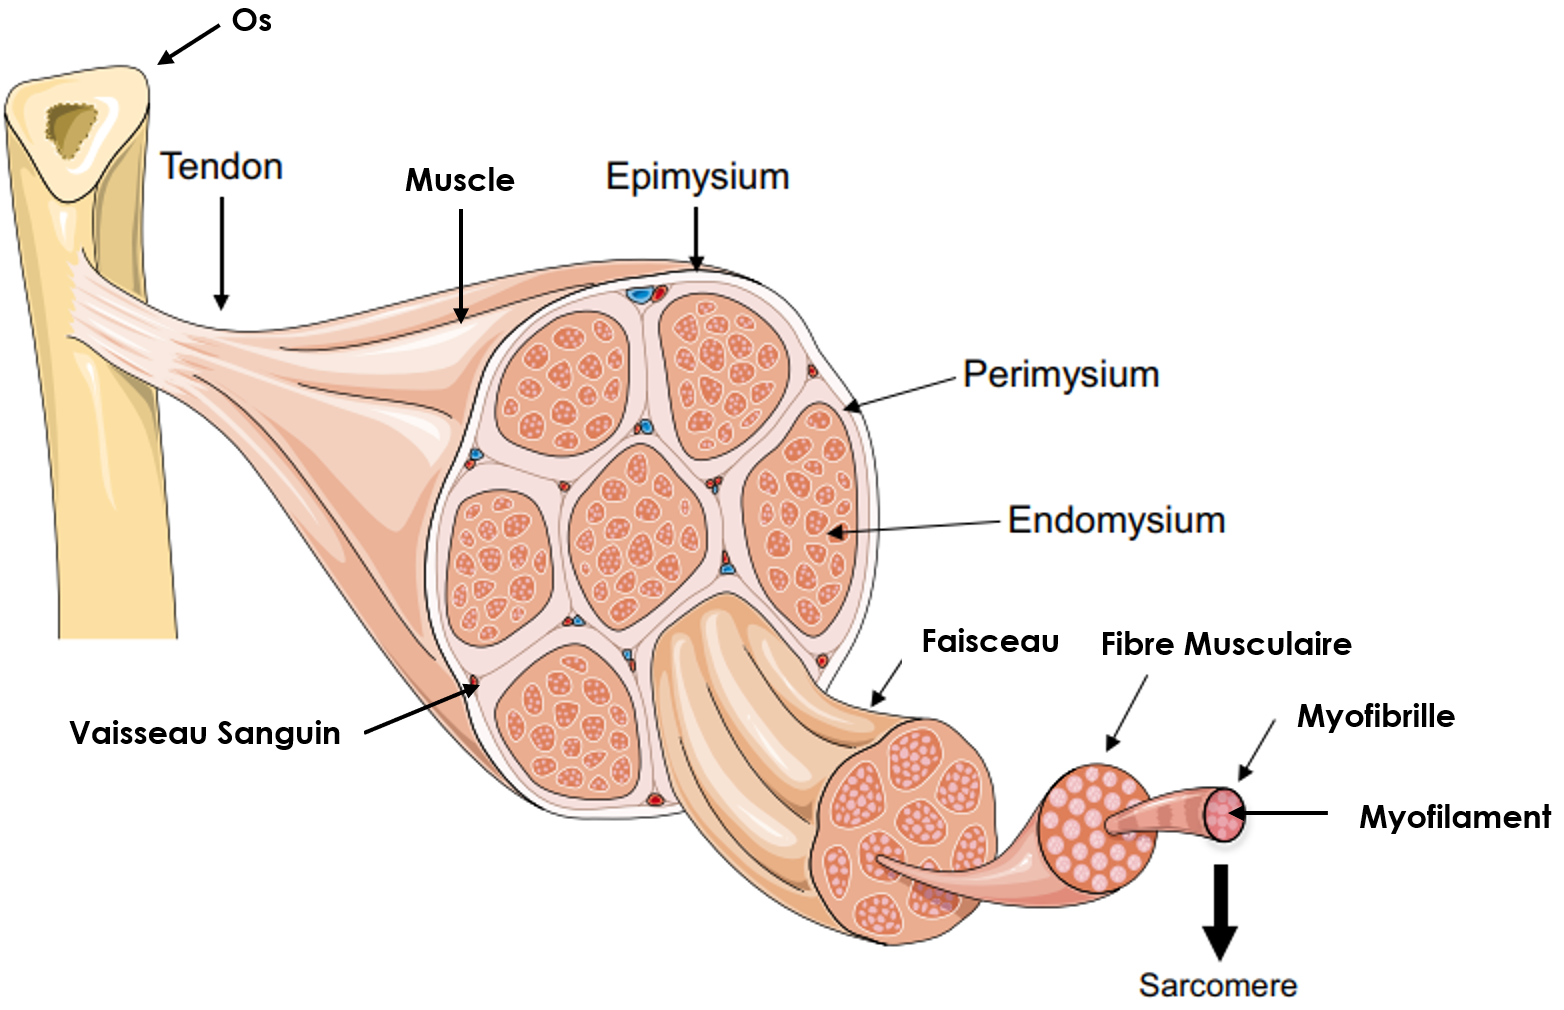
\includegraphics[width=0.8\textwidth]{figures/muscle.png}
 \caption[Schéma de la structure du muscle strié squelettique (modifié de \cite{burr_basic_2019}]{\textbf{Schéma de la structure du muscle strié squelettique}. Le muscle lié à l'os par le tendon est structuré en plusieurs faisceaux entourés par le \textit{perimysium} et l'\textit{epimysium}. Chacun de ces faisceaux est composé de fibres musculaires elles-mêmes composées de myofibrilles et de myofilaments. Dans chacun de ces myofilaments, on retrouve plusieurs sarcomères. (modifiée de \cite{burr_basic_2019}.}
 \label{fig:muscle_struct}
\end{figure}

À une échelle encore plus petite, les myofibrilles sont organisées en plusieurs sarcomères, présentés en figure \ref{fig:sarcomere} (\cite{burr_basic_2019}). Le sarcomère est l'unité contractile de base des myofibrilles. Il est constitué de trois systèmes de filaments protéiques: (i) un filament épais de myosine (ii) un filament mince d'actine inséré sur le disque Z et (iii) un filament élastique enchâssé sur le filament de myosine composé de la titine insérée sur le disque Z aussi.

Lors d'une contraction musculaire, les filaments de myosine et d'actine dans la bande A glissent les uns sur les autres, réduisant ainsi la zone H, le muscle est contracté, le sarcomère est raccourci. On comprend alors qu'un dysfonctionnement dans l'une de trois protéines essentielles à ce mouvement de contraction altère la structure du sarcomère et donc la capacité contractile du muscle. Les gènes TTN, ACTA1 et MYH2/MYH7 (codant respectivement pour la titine, actine et myosine) sont des gènes typiquement responsables de myopathies lorsqu'ils sont mutés. Cependant les gènes impliqués dans le sarcomère ne sont pas les seules pouvant provoquer un dysfonctionnement musculaire, nous verrons l'ensemble des gènes responsables des myopathies congénitales dans une section suivante.
\begin{figure}[!ht]
 \centering
 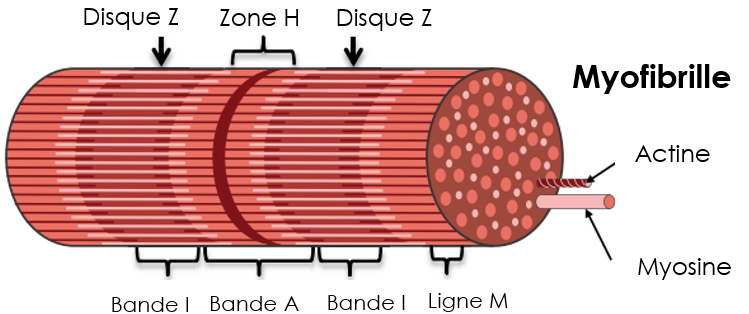
\includegraphics[width=0.75\textwidth]{figures/sarcomere.png}
 \caption[Schéma de la structure du sarcomère.]{\textbf{Schéma de la structure du sarcomère}. Le sarcomère est composé de trois filaments protéiques: un filament épais de myosine, un filament mince d'actine inséré sur le disque Z et un filament élastique de titine et myosine. Par glissement de la myosine sur l'actine dans la bande A, la contraction est rendue possible, raccourcissant la zone H. (modifié de \cite{burr_basic_2019}).}
 \label{fig:sarcomere}
\end{figure}

\subsection{Types de fibres musculaires}
Les fibres musculaires peuvent être classées en trois types de fibres: les fibres de type 1, les fibres de type 2A et 2B qui ont des caractéristiques structurelles et fonctionnelles différentes. Cette classification repose sur le profil d'expression de la chaine lourde de la myosine. Il existe plusieurs isoformes de la myosine (MYH1, MYH2 et MYH7 \cite{tajsharghi_myosinopathies_2013}), permettant chacun une contraction plus ou moins rapide et résistante à la fatigue. Le tableau \ref{table:fiber-compare} répertorie les différences principales entre les fibres de type 1, 2B et 2A.

\begin{table}[!ht]
\centering
\begin{tabular}{|l|c|c|c|} 
 \hline
 \textbf{Caractéristique} & \textbf{Fibre Type 1} & \textbf{Fibre Type 2B} & \textbf{Fibre Type 2A} \\
 \hline
Couleur & Rouge & Pâle & Pâle \\
Vitesse de Contraction & Lente & Rapide & Rapide \\
Voie métabolique & Aérobie & Anaérobie & Aérobie et anaérobie \\
Réserve en oxygène & Importante & Faible & Moyenne \\
Réserve en glycogène & Faible & Importante & Moyenne \\
Fatigabilité & Faible & Importante & Moyenne \\
 \hline
\end{tabular}
\caption[Tableau de comparaison des fibres de type 1, 2B et 2A.]{\textbf{Tableau de comparaison des fibres de type 1, 2B et 2A.} Les fibres de type 1 sont des fibres à contraction lente, endurantes et utilisant le métabolisme aérobie. Les fibres types 2B sont des fibres à contraction rapide, avec faible endurance et à voie métabolique anaérobie. Les fibres de type 2A sont à mi-chemin entre les fibres de type 1 et 2B en termes d'endurance et de vitesse de contraction.}
\label{table:fiber-compare}
\end{table}

Les fibres de type 1, nommées fibres rouges, sont des fibres à contraction lente. Elles ont en général un plus petit diamètre et sont plus vascularisées. Ce sont des fibres spécialisées dans l'aérobie et très résistantes à la fatigue. Elles sont efficaces dans l'utilisation de l'oxygène pour générer de l'\gls{atp} qui est la source d'énergie permettant la contraction musculaire. Leur couleur rouge provient de la présence de myoglobine, la protéine stockant l'oxygène dans le muscle. Ces fibres sont utilisées pour le maintien de la posture et sont mobilisées dans les activités d'endurance à faible intensité.


Les fibres de type 2B sont des fibres à contraction rapide. Ces fibres sont aussi nommées fibres blanches, elles sont spécialisées dans les mouvements rapides et explosifs. Ces fibres utilisent des voies anaérobies pour générer de l'\gls{atp} et se fatiguent beaucoup plus rapidement. La voie anaérobie ne repose pas sur l'oxygène, mais l'utilisation du glycogène. Ces fibres possèdent donc des réserves de glycogène plus importantes que les fibres de type 1. Ces fibres sont mobilisées dans le cadre d'activité intense telle que des sprints.


Enfin, les fibres de type 2A représentent un intermédiaire entre les fibres de type 1 et 2B. Ces fibres peuvent générer de l'énergie (\gls{atp}) à la fois par la voie aérobie et anaérobie. À l'instar des fibres 2B, elles peuvent générer des contractions puissantes, mais se fatiguent rapidement. Ces fibres sont mobilisées lors des exercices à intensité moyenne demandant de l'endurance telle que la natation.


La balance entre fibres type 1 et 2A/2B dans un muscle est un marqueur important des myopathies congénitales. Souvent dans le cadre de myopathies, une prédominance des fibres de type 1 va se manifester dans le muscle. En microscopie, la visualisation de ces fibres se réalise par des méthodes histochimiques telles que la coloration ATPase qui colore différentiellement les fibres de type 1 et fibres de type 2. 

\subsection{Classification des atteintes neuromusculaires}
La variété des processus impliqués dans le fonctionnement normal du muscle strié squelettique ouvre la porte de nombreux dysfonctionnements pouvant amener à une défaillance du muscle. Ces défaillances peuvent provoquer des maladies aux manifestations variées que l'on nomme les \gls{nmd}. Les \gls{nmd} ont une prévalence d'environ 3,7 à 4,9 pour 10 000 (\cite{lace_overview_2022}), ce qui les classe parmi les maladies rares (prévalence inférieure à 5 pour 10 000). Les \gls{nmd} héréditaires affectant les muscles striés squelettiques peuvent être classifiées parmi quatre grandes catégories présentées dans le tableau \ref{table:nmd} (\cite{lornage_identification_2019, benarroch_2023_2023}). Les dystrophies musculaires sont caractérisées principalement par une perte progressive de la force et de la masse musculaire. Les patients atteints de myopathies métaboliques présentent une forte intolérance à l'exercice et des épisodes de fatigue. Les myopathies mitochondriales sont aussi caractérisées par une faiblesse musculaire et une intolérance à l'exercice, mais en plus par des problèmes cardiaques, auditifs et des crises d'épilepsie.

Enfin, les myopathies congénitales, qui sont le sujet principal de notre cas d'application, sont des maladies avec un départ précoce de la faiblesse musculaire (souvent dès la naissance) et dont la progression est lente. De plus, les patients atteints de myopathies congénitales présentent souvent des caractéristiques faciales dysmorphiques (visage, bouche). Dans la prochaine section, nous allons voir en détail la classification et la prévalence des myopathies congénitales ainsi que leur diagnostic.
\begin{table}[!ht]
\centering
\begin{tabularx}{\textwidth}{|X|X|}
 \hline
\multicolumn{1}{|c|}{\textbf{Dystrophies musculaires}} & \multicolumn{1}{|c|}{\textbf{Myopathies métaboliques}} \\
\hline
\begin{itemize}
\item Faiblesse musculaire progressive
\item Perte de masse musculaire
\end{itemize} &
\begin{itemize}
\item Intolérance à l'exercice
\item Épisodes de fatigue
\item Myalgie
\end{itemize} \\
\hline

\multicolumn{1}{|c|}{\textbf{Myopathies mitochondriales}} & \multicolumn{1}{|c|}{\textbf{Myopathies congénitales}} \\
\hline
\begin{itemize}
\item Faiblesse musculaire
\item Intolérance à l'exercice
\item Implication cardiaque
\item Perte auditive
\item Crises d'épilepsie
\end{itemize} &
\begin{itemize}
\item Faiblesse musculaire à départ précoce
\item Progression lente de la maladie
\item Caractéristiques faciales dysmorphiques (visage allongé et palais vouté)
\end{itemize} \\
\hline
\end{tabularx}

\caption[Tableau des différentes atteintes neuromusculaires et leurs caractéristiques principales]{\textbf{Tableau des différentes atteintes neuromusculaires héréditaires et leurs caractéristiques principales}. Il y a quatre grandes classes d'atteintes neuromusculaires héréditaires affectant le muscle strié squelettique. Dans cette thèse, nous nous sommes concentrés sur les myopathies congénitales. (\cite{lornage_identification_2019})}
\label{table:nmd}
\end{table}

\section{Les myopathies congénitales}
\subsection{Description générale}
Les myopathies congénitales (\gls{mc}) sont une famille de maladies génétiques rares qui affectent les muscles en général dès la naissance, mais les premiers symptômes peuvent n'apparaitre qu'à l'adolescence ou à l'âge adulte. Les \gls{mc} se caractérisent principalement par la présence d'anomalies histopathologiques dans la biopsie musculaire indiquant une anomalie de la structure musculaire et de ses capacités contractiles.

Les myopathies congénitales sont des maladies génétiques rares, dont la prévalence d'environ 1,5 pour 100 000 dans la population générale et 2,73 pour 100 000 dans la population pédiatrique (\cite{huang_systematic_2021}). Elles sont donc une prévalence inférieure à 50 pour 100 000, seuil pour considérer une maladie comme rare. La \textit{Muscle Gene Table} (\url{https://www.musclegenetable.fr/}, \cite{benarroch_2023_2023}) référence l'ensemble des gènes responsables et des classes de maladie considérées comme des \gls{nmd}. Sur les 658 gènes référencés, il y a 47 gènes identifiés comme pouvant être responsables de \gls{mc} et cette liste évolue chaque année avec l'identification de nouveaux gènes, ce qui rend le diagnostic génétique complexe. 

\subsection{Approches curatives des myopathies congénitales}
Actuellement, il n'existe aucun traitement curatif autorisé sur le marché contre les \gls{mc}. Des approches curatives sont en cours de développement soit au stade préclinique soit au stade d'étude clinique (\cite{gineste_therapeutic_2023, guan_gene_2016}). Parmi les approches explorées, on retrouve des approches de thérapies géniques, qui consistent à essayer de rétablir la fonction du gène défaillant en introduisant une copie fonctionnelle du gène dans l'organisme. Cette approche est en cours d'étude pour les \gls{mc} liées à une défaillance des gènes ACTA1, MTM1 et DNM2, BIN1, RYR1 et STIM1. Cependant, les thérapies géniques sont très couteuses et complexes à développer et mettre en place. Une seconde approche utilisée est l'utilisation de molécules pharmacologiques pour pallier la fonction défaillante. Ces molécules sont en études précliniques dans de nombreuses \gls{mc}, telles que celle causée par les gènes cités précédemment, ainsi que TPM2, TMP3, NEB et SEPN1. 

Cependant, que ce soit pour la thérapie génique ou l'utilisation de molécules pharmacologiques, les développements restent difficiles, notamment dans le cadre du passage de l'expérimentation animale à l'Homme. La startup strasbourgeoise Dynacure a développé en 2019 une petite molécule, un oligonucléotide antisens, nommée DYN101 pour le traitement des myopathies congénitales centronucléaires liées aux gènes DNM2 et MTM1. Le développement de ce traitement a dû être arrêté suite à une toxicité hépatique trop importante chez l'Homme lors de la seconde phase de l'essai clinique. Cette toxicité n'avait pas été observée dans le modèle murin utilisé.

\subsection{Classification et prévalence}
Les myopathies congénitales sont un groupe de maladies hétérogènes dont le principal critère de classification est la biopsie musculaire. Les myopathies congénitales peuvent être classées en trois sous-types principaux: (i) \gls{com} (ii) \gls{nm} (iii) \gls{cnm} et deux sous-types supplémentaires: (iv) \gls{cftd} et (v) myopathie de stockage de myosine (\textit{myosin storage myopathies}, MSM) (\cite{cassandrini_congenital_2017, claeys_congenital_2020, north_approach_2014}). Dans cette sous-section, nous allons présenter les caractéristiques histologiques et cliniques principales de chaque sous-type ainsi que les gènes impliqués. 

\subsubsection{Myopathies à cores (COM)}
Les myopathies à cores (COM) peuvent se diviser en deux sous-groupes supplémentaires: les myopathies à core unique et central (CCD) et les myopathies à multi-minicores (MmD). Les \gls{com} sont largement associées à différentes mutations dans le gène RYR1 avec des formes dominantes provoquant principalement le sous-type CCD et récessives provoquant principalement le sous-type MmD. Les myopathies à core de type MmD possèdent un terrain génétique plus varié, des mutations dans SEPN1 et MYH7 pouvant aussi être responsables de la maladie (\cite{cassandrini_congenital_2017} ). Ce sous-type de myopathies possède une prévalence d'environ 0,37 pour 100 000 (\cite{huang_systematic_2021}) en faisant la \gls{mc} la plus commune. 


Au niveau histopathologique, les \gls{com} se caractérisent principalement par la présence de cores (présentés en figure \ref{fig:cores}), des zones avec une activité oxydative très réduite. Ces zones sont soit uniques, centrales et de grande taille, soit de petites tailles et multiples dans une même fibre musculaire. De plus, on retrouve moins fréquemment la présence de noyaux centralisés, une disproportion dans le ratio de fibres type 1 et type 2 et la présence d'infiltration du tissu conjonctif (\cite{jungbluth_congenital_2018}). Au niveau clinique, en fonction du gène impliqué, on va retrouver très fréquemment des atteintes des muscles extra-oculaires et des atteintes bulbaires (RYR1 récessif), ainsi que des atteintes respiratoires et cardiaques (SEPN1). Les symptômes des \gls{com} peuvent apparaitre à la naissance, durant l'enfance où à l'âge adulte en fonction du gène impliqué.

\begin{figure}[!ht]
 \centering
 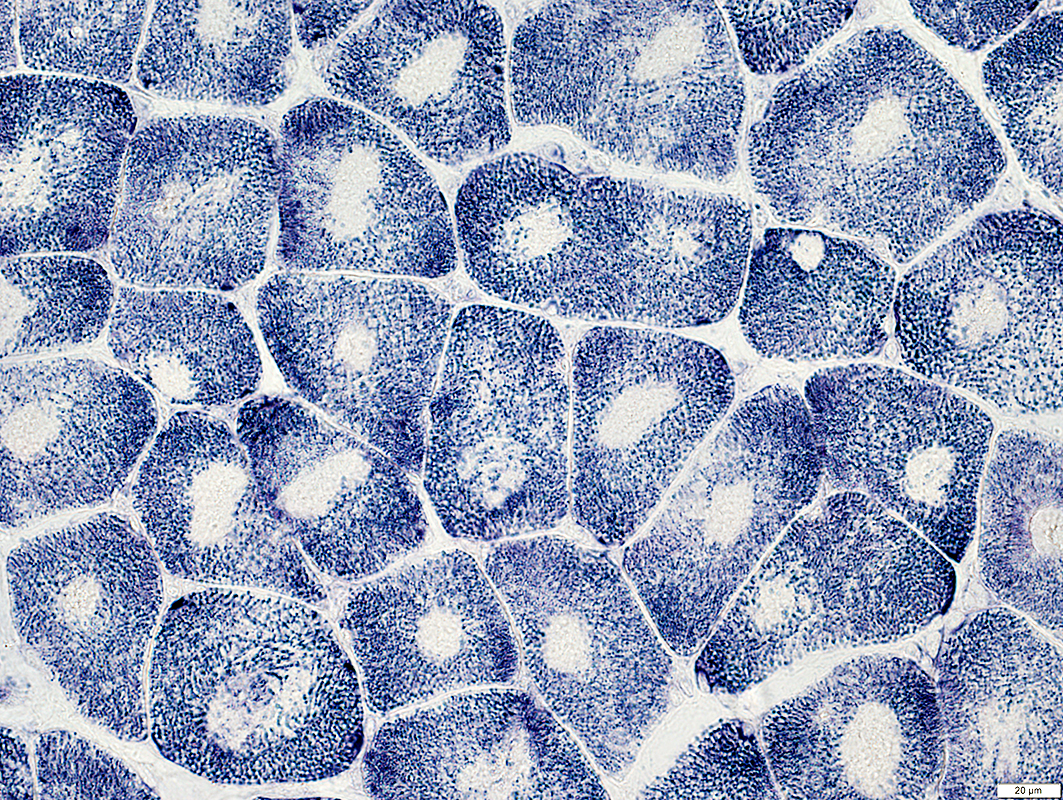
\includegraphics[width=0.5\textwidth]{figures/core.jpg}
 \caption[Biopsie de muscle de myopathies à cores]{\textbf{Biopsie de muscle présentant des cores}. Ces zones à faible activité oxydative sont caractéristiques des myopathies à core à la coloration NADH (\cite{alan_pestronk_neuromuscular_2022})}
 \label{fig:cores}
\end{figure}

\subsubsection{Myopathies à némaline (NM)}
Les myopathies à némaline (NM) sont associées à plus d'une dizaine de gènes, dont le plus communément responsable est NEB (\cite{jungbluth_congenital_2018} ). Ce sous-type de myopathie présente une prévalence de 0,20 pour 100 000 (\cite{huang_systematic_2021}). Au niveau histopathologique, cette myopathie se caractérise principalement par la présence d'inclusions ressemblant à des bâtonnets (illustré en figure \ref{fig:rods}). Il peut aussi y avoir la présence de cores similaires aux \gls{com}. Au niveau clinique, les patients atteints de \gls{nm} présentent des problèmes respiratoires, des contractures et des atteintes bulbaires (\cite{jungbluth_congenital_2018} ), mais pas d'atteinte cardiaque. Les symptômes apparaissent en général dès la naissance et parfois à l'enfance, mais pas à l'âge adulte (\cite{jungbluth_congenital_2018} ).


Les \gls{nm} possèdent un niveau de sous-typage supplémentaire avec deux classes: (i) les myopathies à "cap", une forme très rare de \gls{nm} avec 20 patients décrits entre 1981 et 2017 et (ii) les myopathies nommées "\textit{zebra body}" où le muscle possède une apparence zébrée, qui est une forme de \gls{mc} bénigne avec moins de 10 patients décrits (\cite{cassandrini_congenital_2017}).
\begin{figure}[!ht]
 \centering
 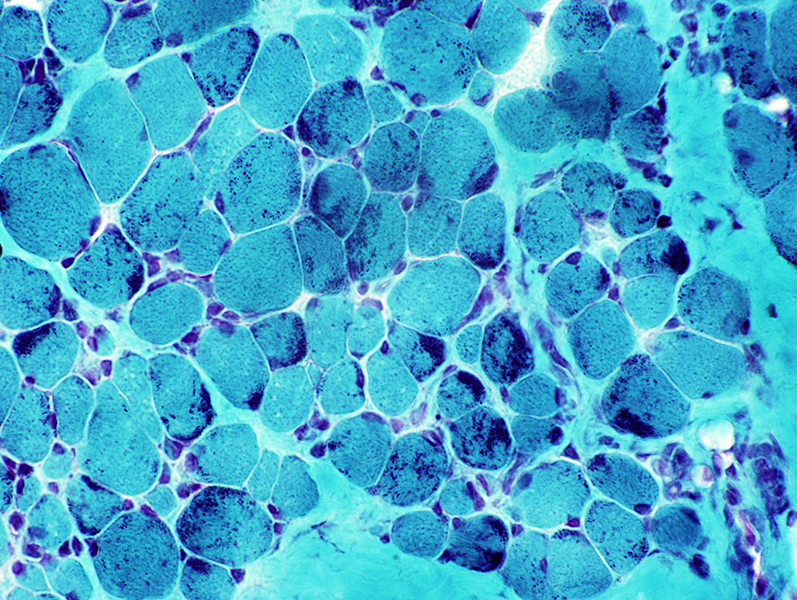
\includegraphics[width=0.5\textwidth]{figures/rods.jpg}
 \caption[Biopsie de muscle de myopathies à némaline]{\textbf{Biopsie de muscle présentant des bâtonnets}. Ces inclusions sombres sont caractéristiques des myopathies à némaline à la coloration trichrome de Gomori (\cite{alan_pestronk_neuromuscular_2022}).}
 \label{fig:rods}
\end{figure}



\subsubsection{Myopathies centronucléaires (CNM)}
Les myopathies centronucléaires (CNM), aussi nommées myopathies myotubulaires, sont des myopathies congénitales plus rares avec une prévalence d'environ 0,08 pour 100 000 (\cite{huang_systematic_2021}). Ce groupe de myopathies peut-être divisé en deux sous-groupes: les \gls{cnm} liées au chromosome X (XLMTM) dû au gène MTM1 et non liées à l'X (DNM2, RYR1, BIN1, TTN...) (\cite{north_approach_2014}). Dans une fibre musculaire saine, les noyaux sont positionnés en périphérie des fibres. Ce groupe de \gls{mc} se caractérise au niveau histopathologique par la présence de noyaux plus gros que la normale, et d'apparence vésiculaire en position centrale des fibres musculaires (présenté en figure \ref{fig:nuc}). De plus, on observe très fréquemment une augmentation de tissus adipeux et conjonctifs dans les fibres de muscles atteints de \gls{cnm} (\cite{jungbluth_congenital_2018}). Concernant les formes de \gls{cnm} liées à l'X, l'atteinte est présente dès la naissance, tandis que pour les formes non liées à l'X l'atteinte se déclare fréquemment à l'âge adulte, notamment dans le cas de DNM2 (\cite{jungbluth_congenital_2018}). Au niveau clinique, on retrouve fréquemment les atteintes des muscles extra-oculaires présentes aussi dans les \gls{com}, les atteintes bulbaires, respiratoires, cardiaques et des contractures. 

\begin{figure}[!ht]
 \centering
 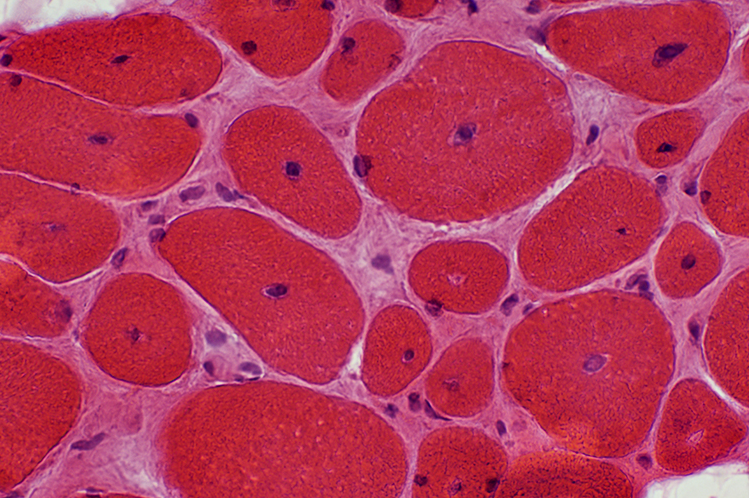
\includegraphics[width=0.5\textwidth]{figures/nuc.png}
 \caption[Biopsie de muscle de myopathie centronucléaire.]{\textbf{Biopsie de muscle présentant des noyaux centralisés}. Ces noyaux centralisés sont caractéristiques des myopathies centronucléaires à la coloration hématoxyline-éosine (\cite{alan_pestronk_neuromuscular_2022}).}
 \label{fig:nuc}
\end{figure}

\subsubsection{Myopathies à disproportion congénitale des fibres (CFTD)}
Les myopathies à disproportion congénitale des fibres (CFTD) sont un sous-type moins bien défini et spécifique que les trois sous-types présentés précédemment (\gls{nm}, \gls{cnm}, \gls{com}) qui ont une prévalence d'environ 0,23 pour 100 000. Ce sous-type est principalement défini par la seule présence d'une prédominance des fibres de type 1 et de leur atrophie d'environ 40\% par rapport aux fibres de type 2 (présenté en figure \ref{fig:cftd}, \cite{claeys_congenital_2020} ). Aucune autre anomalie de structure du muscle n'est présente (tel que les bâtonnets, les cores ou les noyaux centralisés) dans ce sous-type de \gls{mc} (\cite{claeys_congenital_2020}). Au niveau clinique, les enfants atteints présentent une hypotonie et une faiblesse musculaire généralisée dès la naissance ou pendant les premières années. De plus, ils présentent une atteinte importante au niveau des muscles du visage et des épaules ainsi que des problèmes respiratoires (\cite{claeys_congenital_2020} ). Ce sous-type de myopathie est lié à une dizaine de gènes tels que ACTA1, MYH7 et RYR1.
\begin{figure}[!ht]
 \centering
 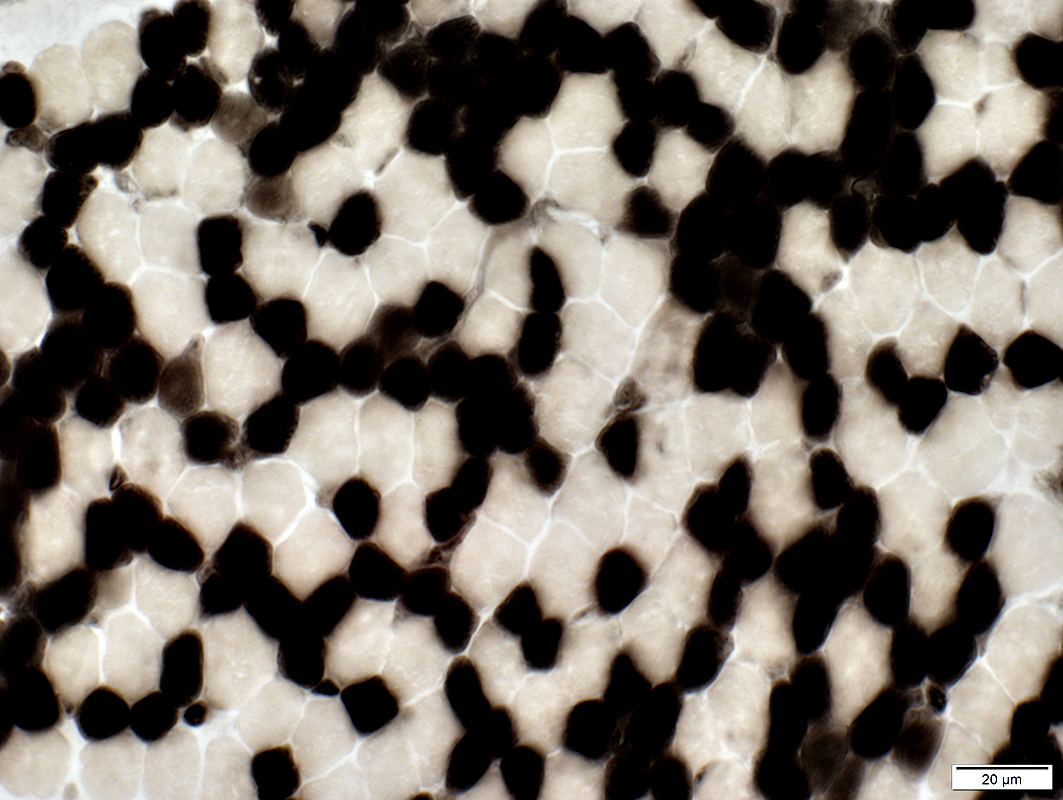
\includegraphics[width=0.5\textwidth]{figures/cftd.jpg}
 \caption[Biopsie de muscle de myopathie à disproportion congénitale des fibres]{\textbf{Biopsie de muscle présentant une atrophie et une prédominance des fibres de type 1}. Cette prédominance est caractéristique des myopathies à disproportion congénitale des fibres à la coloration ATPase pH 4.3 (\cite{alan_pestronk_neuromuscular_2022}).}
 \label{fig:cftd}
\end{figure}
\subsubsection{Myopathies de stockage de myosine (MSM)}
Enfin, les myopathies de stockage de myosine (MSM), anciennement nommées "\textit{hyaline body myopathy}", se caractérisent principalement par la présence de \textit{"hyaline body"}, des régions d'apparence granulaire et basophile à la coloration hématoxyline-éosine (figure \ref{fig:hyaline}, \cite{claeys_congenital_2020, victor_dubowitz_muscle_2020}). Sur le plan clinique, les patients présentent des problèmes cardiaques, une perte de force distale (mains, poignets), des pieds tombants et une pseudo-hypertrophie des mollets (\cite{cassandrini_congenital_2017}). Un seul gène est identifié pour l'instant comme pouvant causer une MSM, il s'agit de MYH7, pouvant aussi causer des \gls{cftd} et des \gls{com}.
\begin{figure}[!ht]
 \centering
 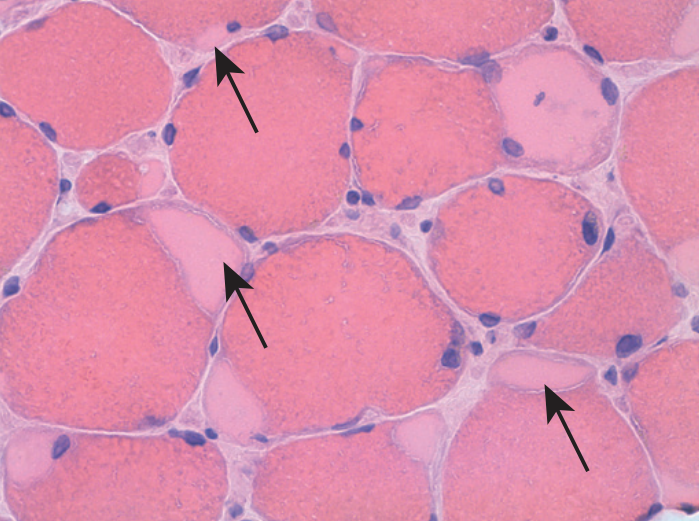
\includegraphics[width=0.5\textwidth]{figures/hyalin.jpg}
 \caption[Biopsie de muscle des \textit{hyaline bodies}]{\textbf{Biopsie de muscle présentant des \textit{hyaline bodies}}. Ces \textit{hyaline bodies} indiqués par les flèches noires sont caractéristiques des myopathies à stockage de myosine (\cite{victor_dubowitz_muscle_2020}).}
 \label{fig:hyaline}
\end{figure}

La diversité des sous-types de myopathies congénitales tant par leur nombre que par leur hétérogénéité intra-sous-type et les recouvrements sur le plan clinique, histologique et génétique entre les sous-types rendent leur diagnostic difficile. Dans la prochaine section, nous verrons quelles sont les stratégies de diagnostic utilisées actuellement et quelles sont les données générées dans le cadre de ce diagnostic.

\section{Le défi du diagnostic des myopathies congénitales}
Les myopathies congénitales présentent une triple diversité importante sur les plans clinique, histopathologique et génétique. Un sous-type de myopathies peut être causé par une mutation dans différents gènes et une mutation dans un gène spécifique peut causer plusieurs sous-types de myopathies, rendant le diagnostic des patients complexe. De plus, une même mutation peut mener à des manifestations différentes d'un point de vue pathologique (\cite{north_approach_2014}). 

Deux approches pour la classification et le diagnostic des \gls{mc} existent (\cite{north_approach_2014}). La première nommée \textit{genotype-up}, consiste à partir de chaque gène responsable de \gls{mc} et à lister l'ensemble des phénotypes (cliniques ou histopathologiques) suggestifs d'une mutation dans ces gènes. La seconde approchée nommée \textit{"phenotype-down"} consiste, à partir des observations cliniques et histopathologiques, à lister les sous-types de myopathies associés et les potentiels gènes candidats pouvant causer ces phénotypes.

Le processus de diagnostic des \gls{mc} se base sur trois niveaux d'informations (cliniques, histopathologiques et génétiques), générant ainsi trois types de données (imagerie, textuelles, et séquences) que nous allons présenter ici pour clore ce chapitre.

\subsection{Séquençage NGS et données de séquences génétiques}
Historiquement, les techniques de séquençage Sanger ont été utilisées pendant des décennies pour identifier les mutations responsables de \gls{mc}. Cependant, les avancées en termes de séquençage grâce aux \gls{ngs}, permettent aujourd'hui de séquencer beaucoup plus rapidement et à bas cout, l'ensemble d'un panel de gènes d'intérêt pour trouver les mutations présentes dans le génome du patient. Cependant, cette approche permettant d'évaluer un grand nombre de gènes simultanément ne résout pas tous les défis de l'identification des mutations causant les myopathies congénitales. En effet, même avec les techniques de \gls{ngs}, 50\% des patients atteints de myopathies congénitales n'ont pas de diagnostic génétique à ce jour montrant qu'il reste un travail à faire pour l'identification de gènes et de mutations responsables de \gls{mc}. Par exemple, le projet MYOCAPTURE, porté par le groupe de recherche de Jocelyn Laporte, est issu d'un consortium de sept équipes de recherche avec pour objectif le séquençage de 1000 exomes de familles atteintes de \gls{nmd} afin d'identifier de nouveaux gènes et mutations.

De plus, comme évoqué précédemment et présenté dans le tableau \ref{tab:gene_myo} (\cite{cassandrini_congenital_2017}), un gène peut être responsable de différents sous-types de \gls{mc}. Les données génétiques seules ne sont donc pas suffisantes pour poser un diagnostic fiable. L'exploitation de ces données de type séquences génétiques requièrent le développement d'outils à même de traiter les résultats de séquençage pour en extraire les mutations, de quantifier la pathogénicité des mutations et de filtrer les mutations pertinentes dans le cadre du diagnostic des \gls{mc}. 

\begin{table}[!ht]
\centering
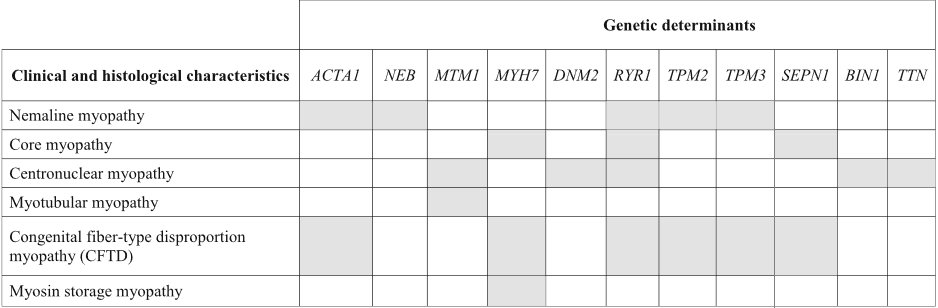
\includegraphics[width=1\textwidth]{figures/gene_tab.png}
\caption[Tableau des principaux gènes responsables de myopathies congénitales et des sous-types associés]{\textbf{Tableau des principaux gènes responsables de myopathies congénitales et des sous-types associés.} Un gène muté peut causer plusieurs types de \gls{mc} et plusieurs types de \gls{mc} peuvent être causées par un même gène. (\cite{cassandrini_congenital_2017})} 
\label{tab:gene_myo}
\end{table}

\subsection{Histopathologie et données d'imagerie }
L'histopathologie est le premier critère de classification des sous-types de \gls{mc}. Comme décrit précédemment, plusieurs marqueurs pathologiques sont à évaluer pour pouvoir orienter le diagnostic des \gls{mc}. Pour observer ces marqueurs, l'examen classique est une biopsie musculaire (pouvant porter sur divers muscles du patient comme le quadriceps, le deltoïde, la vaste externe ou autre) accompagnée d'une observation de la biopsie au microscope sous différentes colorations, fournissant chacune une information sur la structure du muscle. En routine, cinq colorations principales sont réalisées dans le cadre du diagnostic à partir d'une biopsie musculaire: (i) la coloration \gls{he} qui révèle la taille des fibres et la position des noyaux (ii) la coloration \gls{tg} qui révèle la charpente protéique des fibres et qui permet d'observer des agrégats protéiques (iii) la coloration ATPase qui permet de différencier les fibres de type 1 et type 2, et (iv) et (v) les colorations \gls{sdh} et NADH qui révèlent l'activité oxydative des fibres et la position des mitochondries. De plus, des colorations supplémentaires peuvent être réalisées telles que de l'immunohistochimie et les colorations phosphorylases, PAS (glycogène), et Soudan (lipides). Pour finir, dans les cas complexes, il peut être nécessaire d'avoir recours à la microscopie électronique pour observer avec une forte résolution la structure précise des fibres musculaires.

Ainsi, l'examen de la biopsie musculaire génère plusieurs images (une par coloration) de grandes tailles (de l'ordre du millier de fibres par biopsie qui sont évaluées manuellement pour identifier les marqueurs pathologiques. Cependant, comme pour les données génétiques, il est difficile de poser un diagnostic sur la seule base des observations histopathologiques. Comme présenté dans le tableau \ref{tab:histopath} (\cite{jungbluth_congenital_2018}), les caractéristiques typiques d'un sous-type de myopathies, comme les cores dans les myopathies à cores, peuvent être présents dans d'autres sous-types telles que les myopathies à némaline par exemple. Des travaux de recherche sont encore nécessaires pour trouver des critères réellement discriminants entre les sous-types de myopathies sur le plan histopathologique, tel que le projet de l'Atlas du Muscle porté par Bruno Cadot et Norma Romero (\cite{cadot_atlas_2022}). Cet atlas est une banque de données en ligne d'images d'histopathologie de biopsie de muscle dans différentes colorations pour un large panel de \gls{nmd}. À ce jour, plus de 5000 images de biopsies musculaires sont disponibles avec le gène et le diagnostic de \gls{nmd} associés. 

\begin{table}[!ht]
\begin{tabularx}{\textwidth}{|p{1.8cm}|X|X|X|X|X|X|X|X|X|}
 \hline
\textbf{Observation} & \textbf{RYR1 AD} & \textbf{RYR1 AR} & \textbf{SEPN1} & \textbf{TTN} & \textbf{MTM1} & \textbf{DNM2} & \textbf{NEB} & \textbf{ACTA1} & \textbf{KLHL 40} \\
\hline
Cores & +++ & +++ & +++ & ++ & - & + & + & + & - \\
\hline
Noyau central & ++ & ++ & - & +++ & +++ & +++ & - & - & - \\
\hline
Bâtonnets & + & + & - & + & - & - & +++ & +++ & +++ \\
\hline
CFTD & + & +++ & + & + & + & - & - & + & - \\
\hline
Infiltration tissus conjonctifs & ++ & ++ & ++ & +++ & - & + & - & - & - \\
\hline
\end{tabularx}
\caption[Tableau des fréquences des principaux marqueurs pathologiques en biopsie musculaire.]{\textbf{Tableau des fréquences des principaux marqueurs pathologiques observables sur la biopsie musculaire en fonction du gène impliqué.} Un gène muté peut provoquer des phénotypes histologiques spécifiques de différents sous-types de myopathies congénitales. Et chaque phénotype histologique peut être causé par plusieurs gènes différents. (\cite{jungbluth_congenital_2018}).} 
\label{tab:histopath}
\end{table}
L'évaluation des données d'imagerie histopathologique est un processus long en raison du nombre de fibres musculaires et du nombre de colorations. En général, il est réalisé de façon qualitative, sans comptage de fibres et des éléments pathologiques.

\subsection{Comptes rendus cliniques et histopathologiques (données textuelles) }
Les observations cliniques de patients sont aussi un niveau d'information utile et nécessaire au diagnostic des myopathies congénitales. Même si certains phénotypes sont très communs et peu informatifs (hypotonie, faiblesse musculaire générale), d'autres, plus spécifiques, peuvent permettre d'éliminer certains gènes. Le tableau \ref{tab:clinic} (\cite{jungbluth_congenital_2018}) présente la fréquence des principales observations cliniques en fonction du gène impliqué. On observe par exemple que la présence d'une atteinte cardiaque est très fréquente lors d'une mutation du gène TTN, peu fréquentes dans les gènes ACT1, SEPN1 et RYR1 récessif, et totalement absente pour RYR1 dominant, MTM1, DNM2, NEB et KLHL40. Ainsi il est possible d'orienter les tests génétiques et diagnostiques grâce à cette information. Cependant, on observe aussi que ces phénotypes peuvent apparaitre pour de multiples gènes, rendant impossible le diagnostic sur la seule base de critères cliniques. L'observation des phénotypes cliniques, tout comme l'observation des marqueurs histopathologiques, mène à la rédaction d'un compte rendu clinique textuel qui liste les observations réalisées.

\begin{table}[!ht]
\begin{tabularx}{\textwidth}{|p{1.8cm}|X|X|X|X|X|X|X|X|X|}
 \hline
\textbf{Observation} & \textbf{RYR1 AD} & \textbf{RYR1 AR} & \textbf{SEPN1} & \textbf{TTN} & \textbf{MTM1} & \textbf{DNM2} & \textbf{NEB} & \textbf{ACTA1} & \textbf{KLHL 40} \\
\hline
Muscle extra-oculaire & + & +++ & - & - & +++ & +++ & - & - & ++ \\
\hline
Atteinte bulbaire & + & +++ & ++ & ++ & +++ & ++ & ++ & ++ & +++ \\
\hline
Atteinte distale & - & + & - & ++ & + & +++ & ++ & + & + \\
\hline
Atteinte respiratoire & + & ++ & +++ & ++ & +++ & + & ++ & ++ & +++ \\
\hline
Atteinte cardiaque & - & + & + & +++ & - & - & - & + & - \\
\hline
Contractures & + & + & + & +++ & +++ & ++ & ++ & ++ & +++ \\
\hline
\end{tabularx}
\caption[Tableau des fréquences des principales observations cliniques en fonction du gène impliqué]{\textbf{Tableau des fréquences des principales observations cliniques en fonction du gène impliqué.} Comme pour les phénotypes histologiques, un même phénotype clinique peut être provoqué par différents gènes mutés et plusieurs phénotypes cliniques différents peuvent être provoqués par un même gène. (\cite{jungbluth_congenital_2018}).}
\label{tab:clinic}
\end{table}

\section{Conclusions et synthèse de problématiques}
Cette description des myopathies congénitales dresse un portrait complexe du processus de diagnostic, qui requiert l'intégration de trois niveaux d'informations et de modalités différentes (textes, images, séquences). L'ensemble de ces données et leur complexité mettent en avant le besoin d'outils adaptés pour aider à leur exploration automatique. Le but de cette thèse a été de développer des outils capables d'exploiter les comptes rendus et les images de biopsies de patients atteints de myopathies congénitales afin de mieux caractériser les différents sous-types de \gls{mc}.

Pour les comptes rendus de biopsie, ces documents sont très riches en information sur les patients, cependant ils sont dans un format de texte libre rendant difficile leur utilisation informatique. Afin de pouvoir traiter ces données pour en extraire de nouveaux critères de classification, il est nécessaire de développer des outils adaptés à l'annotation, la structuration et la compréhension de texte libre en langage naturel, notamment grâce aux avancées en \gls{ia}. 

Pour les données d'imagerie, comme mentionné précédemment, en raison de leur volume et taille, leur évaluation est souvent réalisée de façon qualitative uniquement. C'est pourquoi il est intéressant de développer des outils capables de réaliser cette évaluation automatiquement de façon quantitative, grâce à des méthodes \gls{ia}. Une approche par \gls{ia} capable de quantifier des éléments sur l'image permet d'extraire des informations plus précises et donc de mieux caractériser et classifier les types de \gls{mc}, par exemple avec la possibilité d'établir des seuils pour les marqueurs pathologiques.

Développer des méthodes permettant d'exploiter les données d'imagerie (biopsie musculaire) et les données textuelles (cliniques et histopathologies) pour mieux caractériser les \gls{mc} et aider à leur classification représente deux défis. Le premier, concerne l'explicabilité et la confiance dans les modèles \gls{ia}, en particulier car il s'agit de données de santé. Il est nécessaire de construire des modèles \gls{ia} explicables et transparents capables d'extraire de la connaissance à partir des données. Le deuxième défi concerne l'exploitation des données en tant que telles en raison de leur complexité (absence de structure, grande dimensionnalité), il est nécessaire d'utiliser des modèles \gls{ia} novateurs tels que les réseaux de neurones profonds pour exploiter ces données.

Pour cela, nous avons développé une stratégie d'exploitation des données mélangeant les méthodes \gls{ml} classiques et les nouvelles technologies \gls{ia}. Les méthodes \gls{ml} classiques permettent de construire des modèles transparents et de confiance capable de réaliser des prédictions et d'extraire des connaissances à partir de données bien structurées et annotées. Les nouvelles technologies \gls{ia} permettent l'extraction d'information de données brutes non structurées, telles que les textes libres et les images. Ainsi en couplant les deux approches il est possible d'utiliser les nouvelles technologies \gls{ia} comme extracteurs d'information à partir des données brutes de patients (une sorte d'annotation automatique) puis d'appliquer les méthodes \gls{ml} classiques explicables et transparentes pour réaliser des prédictions automatiques de diagnostic et extraire des informations liant les observations et le diagnostic.

Dans ce cadre-là, à travers le développement d'\gls{impatient} dans le chapitre 5, nous avons créé une application web et base de données permettant l'annotation manuelle des données textuelles et d'imagerie par ontologie pour pouvoir les exploiter par techniques de \gls{ml} classiques. Dans le chapitre 6, nous avons utilisé différentes techniques de \gls{ml} explicables pour entrainer des modèles de prédiction à partir de cette base de données. De plus, nous avons développé une méthode d'extraction de connaissances à partir d'un de ces modèles. 

Ensuite, dans le chapitre 7, nous avons développé \gls{nlmyo}, un outil basé sur les nouvelles technologies \gls{ia} pour l'exploitation de texte nommée \gls{llms} pour accélérer et automatiser le processus d'annotation, de référencement et de classification des comptes rendus textuels de patients.

Enfin, dans le chapitre 8, nous avons développé \gls{myoquant}, un outil contenant plusieurs méthodes de quantification de marqueurs pathologiques sur les biopsies musculaires de \gls{mc}, basé sur les nouvelles technologies \gls{ia} pour l'imagerie. Cet outil a pour objectif, à terme, de permettre la génération d'un compte rendu de biopsie automatique avec des mesures quantitatives des marqueurs.